\graphicspath{{img/chapter_1/}}

% \begin{savequote}
% ``Trying to reinvent the wheel is a lot of work. It's okay to make some tweaks and enjoy the ride." 
%     \qauthor{Karen Lamb}
% \end{savequote}

\chapter{Introduction}
\label{chapter:introduction}

% \begin{synopsis}
% Background on DM and its current status
% \end{synopsis}
%%%%%%%%%%%%%%%%%%%%%%%%%%%%%%%%%%%%%
%%%%%%%%%%%%%%%%%%%%%%%%%%%%%%%%%%%%%
%%%%%%%%%%%%%%%%%%%%%%%%%%%%%%%%%%%%%

Dark Matter is an enigma in modern physics. Despite the significant scientific
effort that has gone into trying to discern its nature, a definitive detection
proving its existence eludes us. Nevertheless, dark matter's influence 
on our universe is undeniable, with evidence supporting its existence arising on \fixMV{all} scales, large and small.


%%%%%%%%%%%%%%%%%%%%%%%%%%%%%%%%%%%%%
%%%%%%%%%%%%%%%%%%%%%%%%%%%%%%%%%%%%%
%%%%%%%%%%%%%%%%%%%%%%%%%%%%%%%%%%%%%
\section{Evidence for Dark Matter}
%%%%%%%%%%%%%%%%%%%%%%%%%%%%%%%%%%%%%
%%%%%%%%%%%%%%%%%%%%%%%%%%%%%%%%%%%%%
%%%%%%%%%%%%%%%%%%%%%%%%%%%%%%%%%%%%%

Today, the amount of evidence in support of dark matter's existence is overwhelming. This evidence comes from astrophysical and cosmological observations that are inconsistent with a universe composed entirely of visible matter. This section serves as a review of this evidence. 

%%%%%%%%%%%%%%%%%%%%%%%%%%%%%%%%%%%%%
%%%%%%%%%%%%%%%%%%%%%%%%%%%%%%%%%%%%%
\subsection{Astrophysical Observations}
%%%%%%%%%%%%%%%%%%%%%%%%%%%%%%%%%%%%%
%%%%%%%%%%%%%%%%%%%%%%%%%%%%%%%%%%%%%

\subsubsection*{Galaxy Clusters}

Some of the first hints of dark matter's existence came from observations of galaxy clusters. Perhaps the most famous analysis was performed by Fritz Zwicky~\cite{Zwicky:1937zza_MassesNebulaeClusters}, who was puzzled by the high rotational velocities of galaxies within the Coma Cluster. By applying the virial theorem, equating the cluster's kinetic and gravitational potential energies, he found that the cluster would need to contain a much greater amount of \textit{dunkle materie} (dark matter) than visible matter in order to accommodate these high velocities.

\subsubsection*{Rotation Curves of Spiral Galaxies}

The anomalous rotational velocities observed in galaxy clusters can also be observed at the galactic scale. The rotation curves of spiral galaxies, which relate the rotational velocities of stars to their distance from the galactic centre, were observed to be flat at large distances. From the observed distribution of visible matter, Newtonian mechanics predicts that the orbital velocity of a star a distance $r$ from the galactic centre, $v_\star(r)$, is related to the mass of the galaxy, $M(r)$, through
\begin{equation}
    v_\star(r) = \sqrt{\frac{G M(r)}{r}},
\end{equation}
indicating that the velocity should fall off as $1/\sqrt{r}$ at the outer regions of the galaxy where $M(r)$ is constant. Instead, observations of many spiral galaxies indicate that this velocity remains constant out to the edge of the galaxy. 

A simple way to produce such a rotation curve is to introduce a spherically symmetric distribution of dark matter around the galaxy,
\begin{equation}
    \rho_{\mathrm{DM}}(r) = \frac{v_0^2}{4 \pi G r^2},
\end{equation}
that results in a constant rotational velocity of $v_0$ all the way out to the galaxy edge. Detailed simulations of structure formation in a Cold Dark Matter (CDM) universe indicate that the dark matter halo follows a Navaro-Frenk-White (NFW) profile, \fixMV{cite for NFW}
\begin{equation}
    \rho_{\mathrm{DM}}(r) = \frac{\rho_0}{\left( \frac{r}{r_\mathrm{s}}\right)\left( 1 + \frac{r}{r_\mathrm{s}}\right)^2},
\end{equation}
where $\rho_0$ and $r_\mathrm{s}$ are free parameters that must be fit to each individual halo. 
% More detailed simulations show that the true profile deviates slightly from an NFW, instead being more appropriately modeled by an Einasto profile. However, both profiles are observationally indistinguishable.

An example rotation curve for galaxy NGC 6503 is presented in Fig.~\ref{fig:gal_rotn_curve}, with the contributions from each of the matter components to the rotational velocity shown~\cite{Freese:2008cz_may_ReviewObservationalEvidence, Lelli:2016zqa_SPARCMassModels}. As can be seen, the visible matter constituting disk and gas components does not explain the observed rotational velocity. 

\begin{figure}[t!]
    \centering
    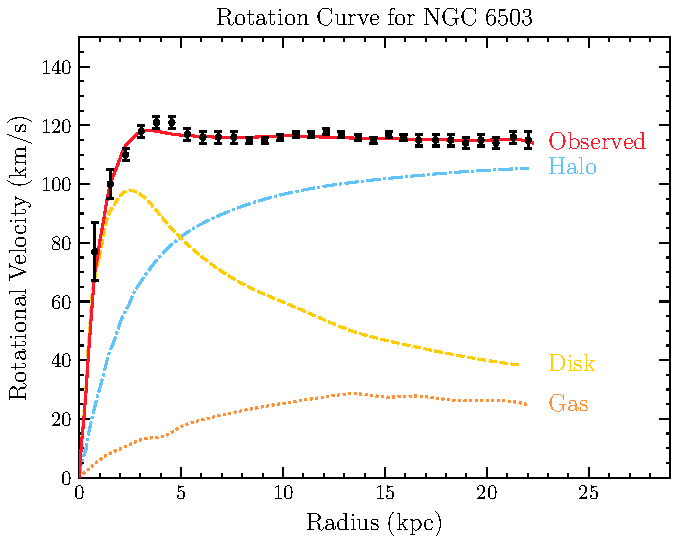
\includegraphics{gal_rotn_N6503}
    \caption{Galaxy rotation curve for NGC 6503, showing the contributions to the total velocity (red) from the DM halo (blue), disk (yellow), and gas components. Data used in making this plot was obtained from~\cite{Freese:2008cz_may_ReviewObservationalEvidence, Lelli:2016zqa_SPARCMassModels}.}
    \label{fig:gal_rotn_curve}
\end{figure}

\subsubsection*{Gravitational Lensing}

As described by General Relativity, the curvature of space-time around massive entities causes light to travel along curved paths. As such, the mass of astrophysical structures can be deduced from the extent to which objects in the background are gravitationally lensed. The disparity between the mass obtained from gravitational lensing and the mass of visible matter in the system is further evidence of dark matter's existence. 

\subsubsection*{The Bullet Cluster}

The bullet cluster is the result of two colliding galaxy clusters which the Chandra X-ray telescope imaged. When viewed in the X-ray, the smearing of the visible matter after the collision is clearly seen, as shown in the red regions of Fig.~\ref{fig:bullet_cluster}, which is expected from such a collision. However, when the gravitational potential was mapped using gravitational lensing, it was clear that the majority of the mass was displaced relative to the visible matter. This mass is attributed to the dark matter components of the original clusters. As indicated by the purple regions in Fig.~\ref{fig:bullet_cluster}, the dark matter halos seem to have passed through each other mostly unperturbed. This tells us that not only is the majority of the mass comprised of dark matter, but that the dark matter has extremely small interactions with both the visible matter and itself. 

\begin{figure}[t!]
    \centering
    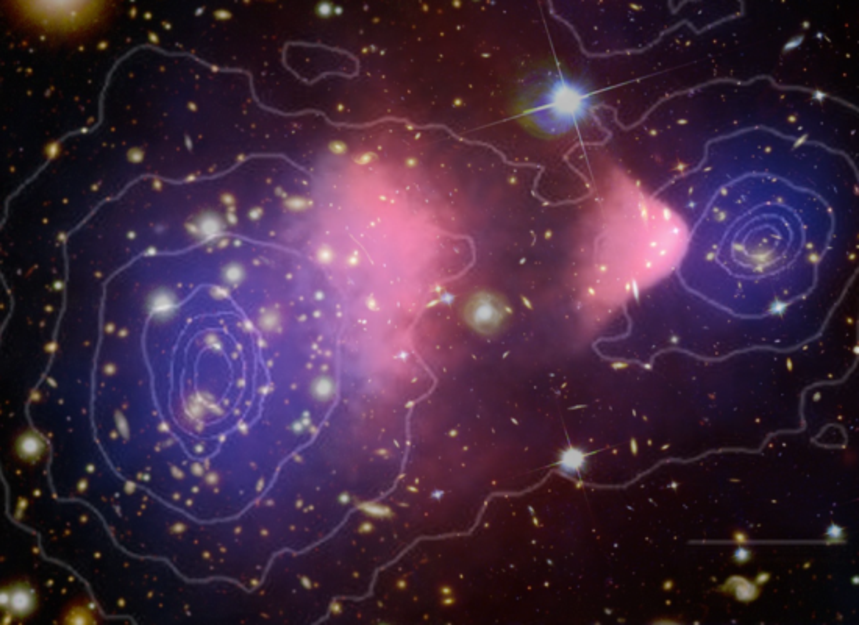
\includegraphics[width = 0.75\textwidth]{bullet_cluster}
    \caption{Image of the Bullet Cluster with contours of the gravitational potential superposed. The red regions indicate the baryonic matter after the collision, while the purple regions are the expected DM components deduced from gravitational lensing. \fixMV{cite}}
    \label{fig:bullet_cluster}
\end{figure}

%%%%%%%%%%%%%%%%%%%%%%%%%%%%%%%%%%%%%
%%%%%%%%%%%%%%%%%%%%%%%%%%%%%%%%%%%%%
\subsection{Cosmological Evidence}
%%%%%%%%%%%%%%%%%%%%%%%%%%%%%%%%%%%%%
%%%%%%%%%%%%%%%%%%%%%%%%%%%%%%%%%%%%%

Dark matter has played a major role in the cosmological history of our universe. The current best cosmological model is the $\Lambda$-Cold Dark Matter model ($\Lambda$CDM), in which cold (i.e. non-relativistic) dark matter plays a prominent role. The relative amount of dark matter present in our universe can be determined with measurements of the light element abundances produced via Big Bang Nucleosynthesis (BBN).

\subsubsection*{The Cosmic Microwave Background}
One of the best probes of cosmological models is the Cosmic Microwave Background (CMB). The CMB is the radiation that was emitted during recombination when the universe had cooled enough for electrons and protons to combine and not be ionised by the photon bath. While the CMB temperature looks isotropic on large scales, fluctuations around the average value of $T_\mathrm{CMB} \sim 2.73\K$ are observed at very small scales. 
These anisotropies are the result of oscillations in the baryonic matter known as Baryon Acoustic Oscillations (BAO). These oscillations were produced due to the interplay between the outward pressure caused by matter interactions and the pull of gravitation due to dark matter. 

Measuring the angular power spectra of these anisotropies and fitting the cosmological parameters of the $\Lambda$CDM model tell us how the universe's energy density ($\Omega_\mathrm{total}$), is partitioned between the matter ($\Omega_\mathrm{m}$), radiation  ($\Omega_\mathrm{rad}$), and dark energy  ($\Omega_\Lambda$) components. In a flat universe, of which we believe ours to be, these components should sum to $\Omega_\mathrm{tot} = 1$.
The Planck collaboration most recently performed a precise measurement of the CMB power spectrum in 2018, obtaining best-fit parameters
\begin{equation}
    \Omega_\mathrm{m} = 0.311 \pm 0.006,\quad \Omega_\Lambda = 0.689 \pm 0.006.
\end{equation}

Combining the predicted baryon density from BBN with the CMB observations breaks down the matter abundance into the dark ($\Omega_\mathrm{DM}$)  and baryonic ($\Omega_\mathrm{b}$) components yielding
\begin{equation}
    \Omega_\mathrm{DM}h^2 = 0.1193 \pm 0.0009,\quad \Omega_\mathrm{DM}h^2 = 0.02242 \pm 0.00014,
\end{equation}
where $h$ is the dimensionless Hubble constant such that the Hubble parameter today is $H_0 = 100\, h\km\s^{-1}\;\mathrm{Mpc}$. 

\subsubsection*{Large Scale Structure}
After recombination, the pressure on the baryonic matter from photons subsided, allowing the small density perturbations to grow. This would lead to the growth of stars, galaxies and the large scale structure we observe today~\cite{Springel:2006vs_LargescalestructureUniverse}. N-body simulations of the universe's evolution require a cold dark matter component for this structure to form. While a small component of the dark matter can be warm, hot dark matter would wash out small scale structures~\cite{Springel:2005nw_Simulatingjointevolution}.  

%%%%%%%%%%%%%%%%%%%%%%%%%%%%%%%%%%%%%
%%%%%%%%%%%%%%%%%%%%%%%%%%%%%%%%%%%%%
%%%%%%%%%%%%%%%%%%%%%%%%%%%%%%%%%%%%%
\section{Potential Models of Dark Matter}
%%%%%%%%%%%%%%%%%%%%%%%%%%%%%%%%%%%%%
%%%%%%%%%%%%%%%%%%%%%%%%%%%%%%%%%%%%%
%%%%%%%%%%%%%%%%%%%%%%%%%%%%%%%%%%%%%

The general consensus amongst physicists is that dark matter has a particle nature, similar to the visible matter of the Standard Model. Models may be as simple as dark matter being described by a single field or there could be an extensive hidden sector with complicated symmetry structures. Given the few details we know about dark matter, there exists an enormous library of models that can produce a viable dark matter candidate. However, there are generic properties a good dark matter candidate must satisfy, namely:

\begin{itemize}
    \item \textbf{Stable on Cosmological Timescales:} Dark matter must either be stable, or have a lifetime significantly longer than the age of the Universe, in order to be present in its current abundance. 
    
    \item \textbf{Neutral or Milli-charged under Electromagnetism:} Dark matter, as its name suggests, does not significantly interact with light. By requiring that dark matter be completely decoupled from the Standard Model plasma by the time of recombination yields an upper bound on the milli-chage dark matter can carry of~\cite{McDermott:2010pa_TurningLightsHow} 
    \begin{equation}
        q_\mathrm{DM}/e < \begin{cases}
            3.5\times10^{-7} \left( \frac{m_\mathrm{DM}}{1\GeV}\right)^{0.58},\quad m_\mathrm{DM} > 1\GeV\\
            4.0\times 10^{-7}\left( \frac{m_\mathrm{DM}}{1\GeV}\right)^{0.35},\quad m_\mathrm{DM} <1\GeV,
        \end{cases}
    \end{equation}
    
    \item \textbf{Small Self-Interactions:} The standard $\Lambda$CDM cosmology assumes that the dark matter is collisionless. However, small dark matter self-interactions can help resolve existing small scale structure issues~\cite{Tulin:2017ara_feb_DarkMatterSelfinteractionsTulin:2017ara_feb_DarkMatterSelfinteractions, Spergel:1999mh_Observationalevidenceselfinteracting}. Current limits on the self-interaction cross section are $\sigma_{\mathrm{DM-DM}}/m_\mathrm{DM} < 0.48\cm^2/\mathrm{g}$ come from merging galaxy clusters~\cite{Randall:2008ppe_ConstraintsSelfInteractionCrossSection} and the ellipticity of galaxies obtained from X-ray observations~\cite{Buote:2002wd_ChandraEvidenceFlattened}.
\end{itemize}

A selection of the more well known dark matter candidates is shown in Fig.~\ref{fig:DM_models_landscape}. We discuss a few of these models below.

\begin{figure}[t!]
    \centering
    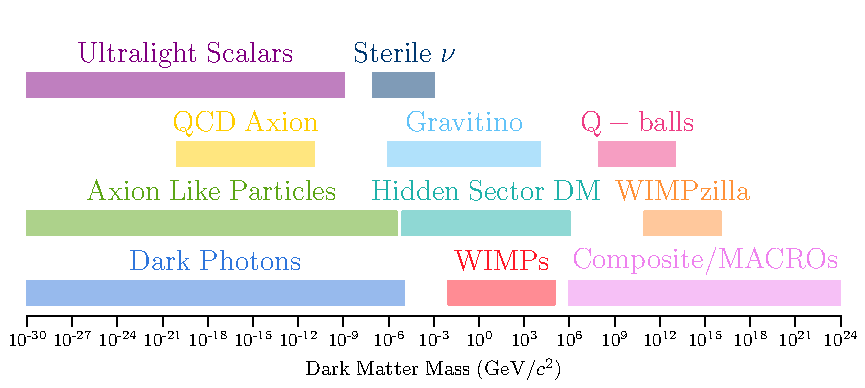
\includegraphics{DM_model_landscape}
    \caption{Illustrative landscape of dark matter models and the mas ranges they predict a valid candidate.}
    \label{fig:DM_models_landscape}
\end{figure}

\subsubsection*{WIMPs}
The Weakly Interacting Massive Particle (WIMP) is perhaps the most well-known dark matter candidate. WIMPs rose to fame thanks to the so-called ``WIMP miracle"~\cite{Feng:2010gw_DarkMatterCandidates}. This refers to the fact that particles with weak scale masses and annihilation cross sections just so happen to have the correct relic abundance of dark matter when produced via the freeze-out mechanism~\cite{Jungman:1995df_Supersymmetricdarkmatter}. In this scenario, the final WIMP abundance depends on the total annihilation cross-section, $\langle\sigma v\rangle$, with only a very mild dependence on the DM mass~\cite{Steigman:2012nb}, 
\begin{equation}
    \Omega_{\mathrm{DM}}h^2 \sim 0.12 \; \left(\frac{2.2\times 10^{-26}\cm^3 \s^{-1}}{\langle \sigma v\rangle}\right).
\end{equation}

The canonical weak-scale WIMP has been tightly constrained from direct and indirect detection limits, leading it to be disfavoured as a dark matter candidate. The term ``WIMP"  is now typically used to refer to any particle dark matter candidate that is produced thermally in the early universe. Such a particle can have a mass in the range $10\MeV\lesssim m_\mathrm{WIMP} \gtrsim 100\TeV$. Lighter WIMPs will have non-negligible contributions to the effective number of neutrino species, $N_{eff}$, which is constrained through BBN and the Cosmic Microwave Background CMB to be $N_{eff} = 2.99 \pm 0.17$~\cite{Planck:2018vyg_sep_Planck2018results}. Masses larger than $\sim 100\TeV$ are excluded from partial wave unitarity~\cite{Griest:1989wd_UnitarityLimitsMass}. 

\subsubsection{Axions}

The original axion was proposed by by Peccei and Quinn~\cite{Peccei:1977hh_CPConservationPresence} as part of a dynamical solution to the ``Strong CP Problem". This refers to the measured value of the neutron electric dipole moment (nEDM) being anomalously small, with a current upper bound of $|d_n| < 0.18\times 10^{-26}\;e\cm$~\cite{Abel:2020pzs_feb_MeasurementPermanentElectric}. This can be translated to an upper bound on the CP-violating QCD $\theta$-parameter such that $|\theta_{QCD}|\lesssim 10^{-10}$, raising questions as to why this value seems to be fine-tuned to such a small value. 

The Peccei-Quinn solution to this problem introduces a new, anomalous, global  $U(1)_{\mathrm{PQ}}$ symmetry, and promote $\theta_\mathrm{QCD}$ to be a dynamical field.
The axion emerges as the pseudo-Goldstone boson associated with the breaking of $U(1)_\mathrm{PQ}$, such is in the two most prominent UV completions of the axion, the KSVZ~\cite{Kim:1979if_WeakInteractionSinglet, Shifman:1979if_CanConfinementEnsure} and DFSZ~\cite{_PossibleSuppressionAxion, Dine:1981rt_SimpleSolutionStrong} models. In these models, the axion produced in the early universe can serve the role of cold dark matter today. This makes it a very compelling dark matter candidate, as it solves two of the biggest mysteries of physics in one neat package. 

Solving the Strong CP problem can be rather restrictive on the model parameters however. For example, the QCD axion's coupling to the photon is not a free parameter, and depends on the scale at which the PQ symmetry is broken. Therefore, many models introduce a light pseudoscalar particle that is not associated with a solution to the Strong CP problem, but has a coupling to the photon that takes the same form as the QCD axion. Such pseudoscalars are known as ``Axion Like Particles" (ALPs), and can similarly make a good dark matter candidate.



%%%%%%%%%%%%%%%%%%%%%%%%%%%%%%%%%%%%%
%%%%%%%%%%%%%%%%%%%%%%%%%%%%%%%%%%%%%
\subsection{Dark Matter in an Effective Fields Theory Framework}
%%%%%%%%%%%%%%%%%%%%%%%%%%%%%%%%%%%%%
%%%%%%%%%%%%%%%%%%%%%%%%%%%%%%%%%%%%%

Given the sheer quantity of potential dark matter models and candidates, 

%%%%%%%%%%%%%%%%%%%%%%%%%%%%%%%%%%%%%
%%%%%%%%%%%%%%%%%%%%%%%%%%%%%%%%%%%%%
%%%%%%%%%%%%%%%%%%%%%%%%%%%%%%%%%%%%%
\section{Current Status of Dark Matter Constraints}
%%%%%%%%%%%%%%%%%%%%%%%%%%%%%%%%%%%%%
%%%%%%%%%%%%%%%%%%%%%%%%%%%%%%%%%%%%%
%%%%%%%%%%%%%%%%%%%%%%%%%%%%%%%%%%%%%



%%%%%%%%%%%%%%%%%%%%%%%%%%%%%%%%%%%%%
%%%%%%%%%%%%%%%%%%%%%%%%%%%%%%%%%%%%%
\subsection{Collider Bounds}
%%%%%%%%%%%%%%%%%%%%%%%%%%%%%%%%%%%%%
%%%%%%%%%%%%%%%%%%%%%%%%%%%%%%%%%%%%%


%%%%%%%%%%%%%%%%%%%%%%%%%%%%%%%%%%%%%
%%%%%%%%%%%%%%%%%%%%%%%%%%%%%%%%%%%%%
\subsection{Direct Detection Searches}
%%%%%%%%%%%%%%%%%%%%%%%%%%%%%%%%%%%%%
%%%%%%%%%%%%%%%%%%%%%%%%%%%%%%%%%%%%%

\begin{figure}
    \centering
    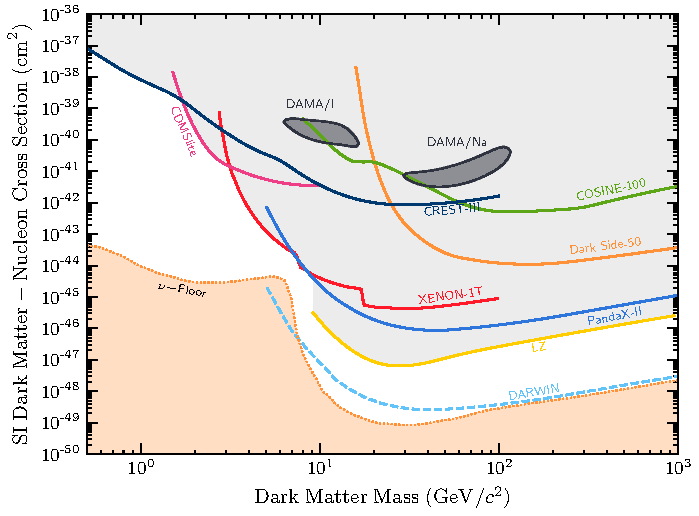
\includegraphics{img/chapter_1/DM_limits_SI.pdf}
    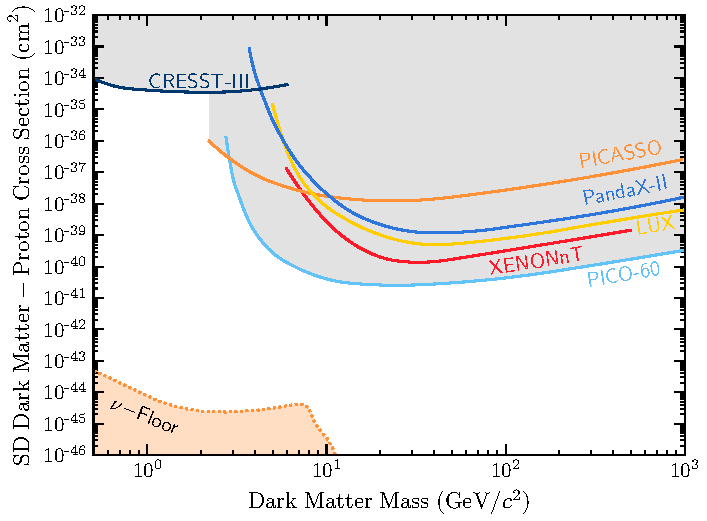
\includegraphics{img/chapter_1/DM_limits_SD_p.pdf}
    \caption{Current status of direct detection limits on spin-independent DM-nucleon (top) and spin-dependent DM-proton (bottom) scattering.}
    \label{fig:direct_detection_lims}
\end{figure}
%%%%%%%%%%%%%%%%%%%%%%%%%%%%%%%%%%%%%
%%%%%%%%%%%%%%%%%%%%%%%%%%%%%%%%%%%%%
\subsection{Indirect Detection}
%%%%%%%%%%%%%%%%%%%%%%%%%%%%%%%%%%%%%
%%%%%%%%%%%%%%%%%%%%%%%%%%%%%%%%%%%%%


It is this route that we will follow to explore dark matter EFTs.

%%%%%%%%%%%%%%%%%%%%%%%%%%%%%%%%%%%%%
%%%%%%%%%%%%%%%%%%%%%%%%%%%%%%%%%%%%%
%%%%%%%%%%%%%%%%%%%%%%%%%%%%%%%%%%%%%
\section{Compact Objects as Dark Matter Probes}
%%%%%%%%%%%%%%%%%%%%%%%%%%%%%%%%%%%%%
%%%%%%%%%%%%%%%%%%%%%%%%%%%%%%%%%%%%%
%%%%%%%%%%%%%%%%%%%%%%%%%%%%%%%%%%%%%


Compact objects, namely Neutron Stars and White Dwarfs, offer a unique
laboratory for studying dark matter interactions. Their extreme environments
offer many benefits in comparison to direct detection experiments. 
These include:

\begin{itemize}
\item \textbf{Gravitational focusing of the DM flux.} In the NS case, the 
infalling DM will be boosted to semi-relativistic velocities ($\sim 0.2 - 0.7 c$
depending on the NS mass).
\item 
\end{itemize}


\begin{figure}
    \centering
    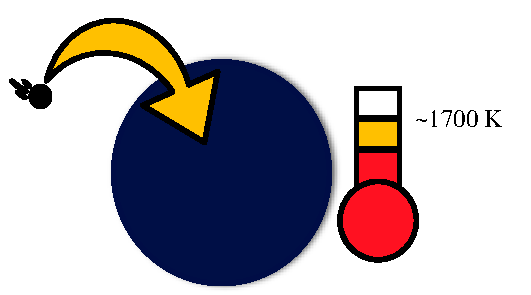
\includegraphics[width=0.45\textwidth]{img/chapter_1/kin_heat_NS.pdf}
    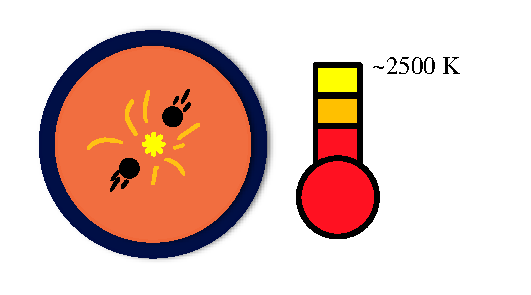
\includegraphics[width=0.45\textwidth]{img/chapter_1/ann_heat_NS.pdf}
    \caption{Illustration of DM-induced heating of compact objects. \textbf{Left:} kinetic heating due to DM scattering, raising the temperature to $\sim 1700 \K$. \textbf{Right:} further annihilation heating adding an additional $\sim 800\K$.}
    \label{fig:cartoon_NS_heat}
\end{figure}




